\documentclass{article}
\usepackage{multicol}
\usepackage[utf8]{inputenc}
\usepackage{graphicx}
\usepackage{geometry}
\PassOptionsToPackage{hyphens}{url}\usepackage{hyperref}

 \geometry{
 a4paper,
 left=20mm,
 right=20mm
 }

\DeclareGraphicsExtensions{.png,.pdf. jpg}

\title{\vspace{-4cm}Thorlabs Post Holder Bases}
\date{}
\begin{document}

\maketitle

\vspace{-1cm}

Last updated: \today

URL: \url{https://www.thorlabs.hk/newgrouppage9.cfm?objectgroup_ID=47}

\begin{multicols}{2}

\section{Brief description}

Baseplates with slots that can be locked down to the optical breadboard with a 1/4 screw and washer.

We usually use the BA1 baseplates, imperial. These have two slots and it's easier to fix the baseplate along the breadboard holes. We also have some of the BA1S plates.

%What the devil. We can fix anything. Those great big fluffy clouds. We have no limits to our world. We're only limited by our imagination. Put it in, leave it alone. Everything's not great in life, but we can still find beauty in it.

%Just let this happen. We just let this flow right out of our minds. That's why I paint - because I can create the kind of world I want - and I can make this world as happy as I want it. This is the fun part How to paint. That's easy. What to paint. That's much harder.

%\section{Picture}

\section{Technical Specifications}


\begin{center}
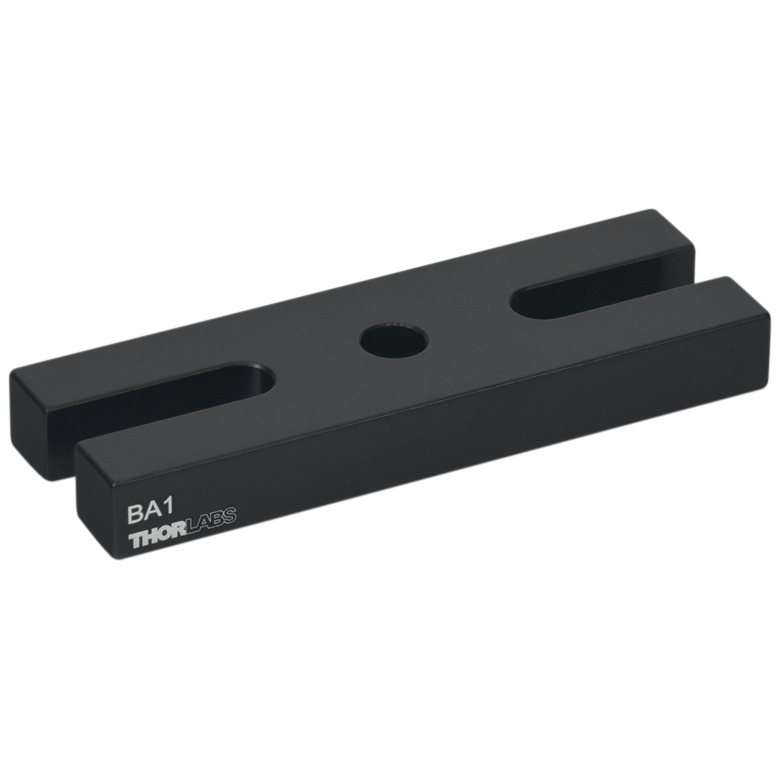
\includegraphics[width=4.3cm]{assets/ba1.jpg}
\end{center}

\noindent BA1

\begin{tabular}{|l|l|}
Slots & 1 \\
Slot length & 0.81'' (20.1 mm)\\
Dimensions & 1'' x 3'' x 3/8'' (25 x 75 x 10 mm)\\
\end{tabular}%

\begin{center}
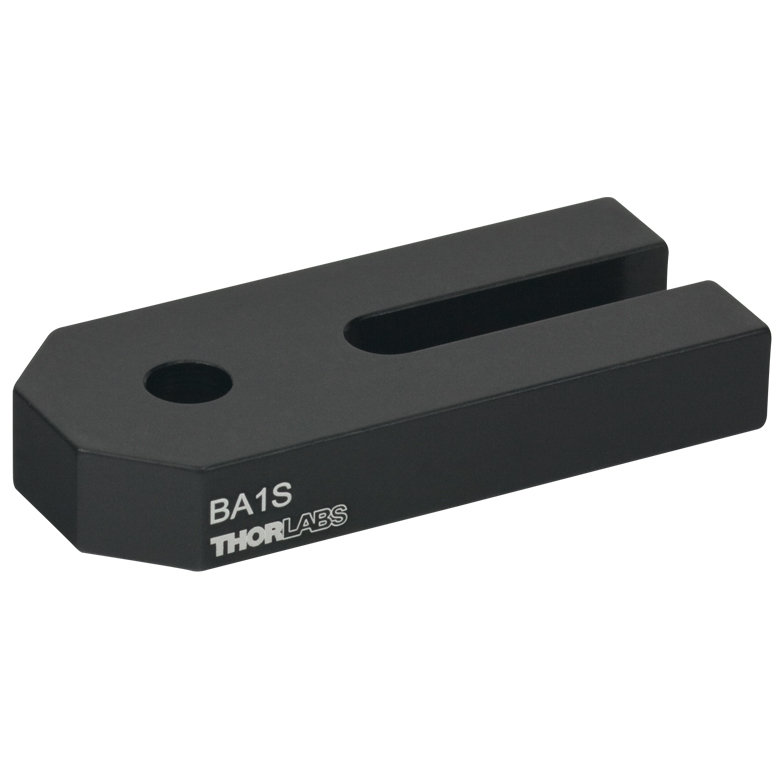
\includegraphics[width=4.3cm]{assets/ba1s.jpg}
\end{center}

\noindent BA1S

\begin{tabular}{|l|l|}
Slots & 1\\
Slot length & 1.10'' (27.9 mm)\\
Dimensions & 1'' x 2.3'' x 3/8'' (25 x 58 x 10 mm)\\
\end{tabular}%

\begin{center}
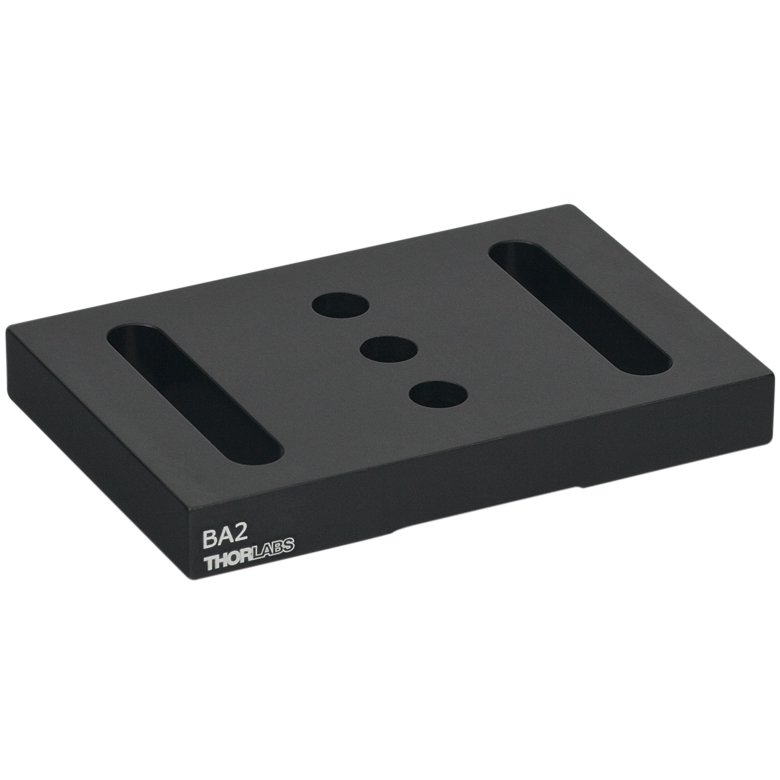
\includegraphics[width=4.3cm]{assets/ba2.jpg}
\end{center}

\noindent BA2

\begin{tabular}{|l|l|}
Slots & 2\\
Slot length & 1.25'' (31.8 mm)\\
Dimensions & 2'' x 3'' x 3/8'' (50 x 75 x 10 mm)\\
\end{tabular}%



%\section{Other notes}

\end{multicols}

\begin{center}
\includegraphics[width=15cm]{assets/cadba1.pdf} \\
\textsf{BA1}
\end{center}

\begin{center}
\includegraphics[width=15cm]{assets/cadba1s.pdf} \\
\textsf{BA1S}
\end{center}

\begin{center}
\includegraphics[width=15cm]{assets/cadba2.pdf} \\
\textsf{BA2}
\end{center}

\end{document}
